\chapter{Architecture}

\section{Overview}

\begin{figure}[h]
    \caption{Overview}
    \centering
    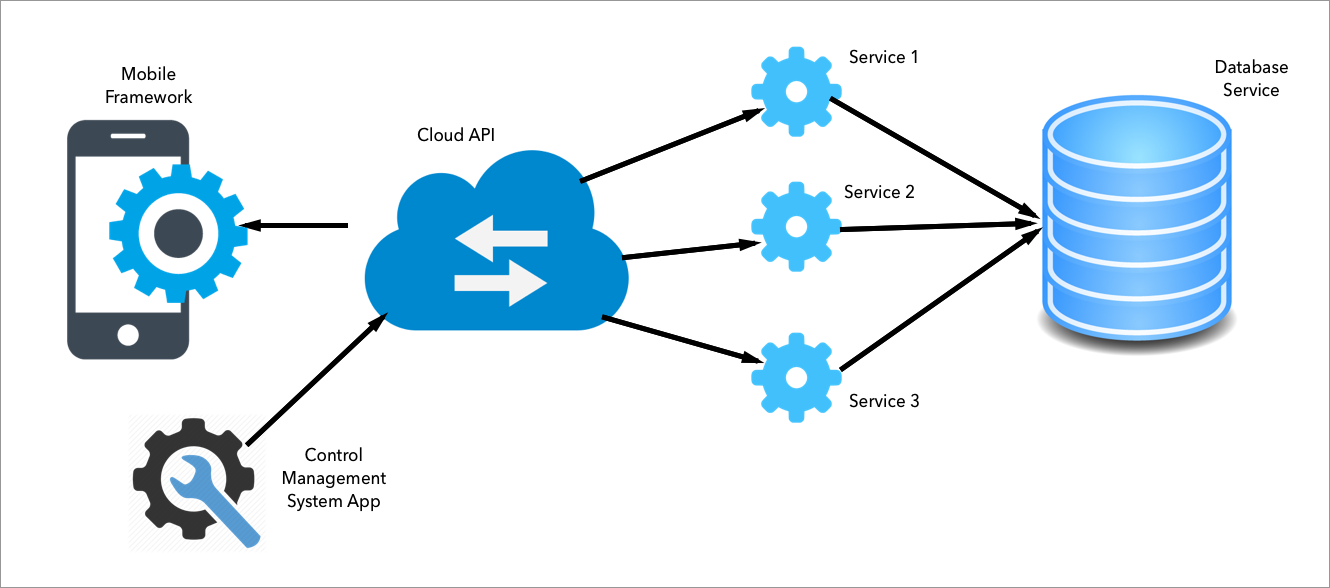
\includegraphics[width=100mm]{images/overview}
    \label{fig:label}
\end{figure}

Fig 4.1 shows the complete Mobile Back-end as a Service system. It shows the mobile framework used by developers application to send HTTPS request using a REST API such as get request to retrieve objects from the database layer using a service layer. The service layer is where the database, notifications
and remote configuration services sit. So when a request is made to the Cloud Rest API framework such as send object to the server , the API will call the database service class and will enter the object into the database and return the result back to the client ( framework). The diagram also shows the Control Management System (CMS) app using a dashboard to accomplish such tasks as send the configuration files updates to the server, which will send HTTPS request to the Cloud API and have its own service class to accomplish these tasks. The diagram only displays 3 service class, but can be as many as required.

\begin{figure}[h]
    \caption{Framework Overview}
    \centering
    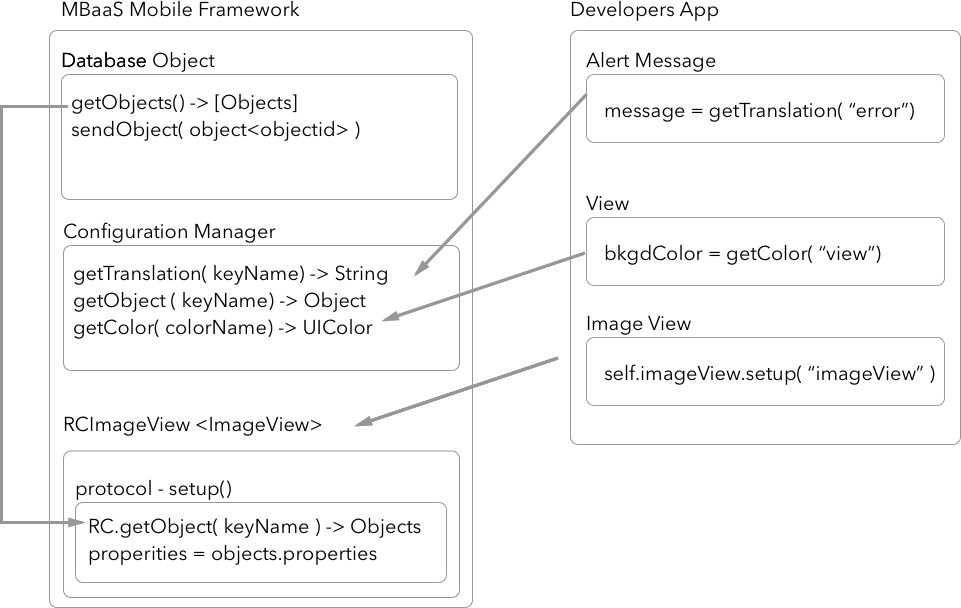
\includegraphics[width=100mm]{images/framwork_architecture}
    \label{fig:label}
\end{figure}

Mobile frameworks separates the back-end API by functionality, making it easier for developers to create apps without having to learn how the API works. It provides class functions and protocols to which can be used to interact with the server API. An example of this is in Fig 5.3 where the framework has the database object that makes HTTPS request to retrieve the objects, but the developer can use the inherited function call getObjects. The
remote configuration requests are also in the diagram to get values from the JSON files stored on the mobile phone app directory.


\section{Diagram}

\section{Development Concepts}
